\documentclass[12pt,a4paper]{article}

\usepackage[utf8]{inputenc}
\usepackage[T2A]{fontenc}
\usepackage[ukrainian]{babel}
\usepackage{geometry}
\geometry{left=2cm,right=2cm,top=2cm,bottom=2cm}

\usepackage[table]{xcolor}
\usepackage{array}
\usepackage{amsmath}
\usepackage{graphicx}
\usepackage{minted}
\usepackage{float}
\usepackage{tikz}
\usetikzlibrary{arrows.meta,positioning}
\usepackage{hyperref}

\usemintedstyle{vs}
\setminted{linenos,breaklines,frame=single,fontsize=\small}

\hypersetup{
  unicode=true,
  pdftitle={ДКР з цифрової схемотехніки},
  pdfauthor={Давидчук Артем, Дубров Дмитро},
  pdfsubject={Розроблення модулів арифметико-логічних блоків}
}

\begin{document}

\begin{titlepage}
    \begin{center}
        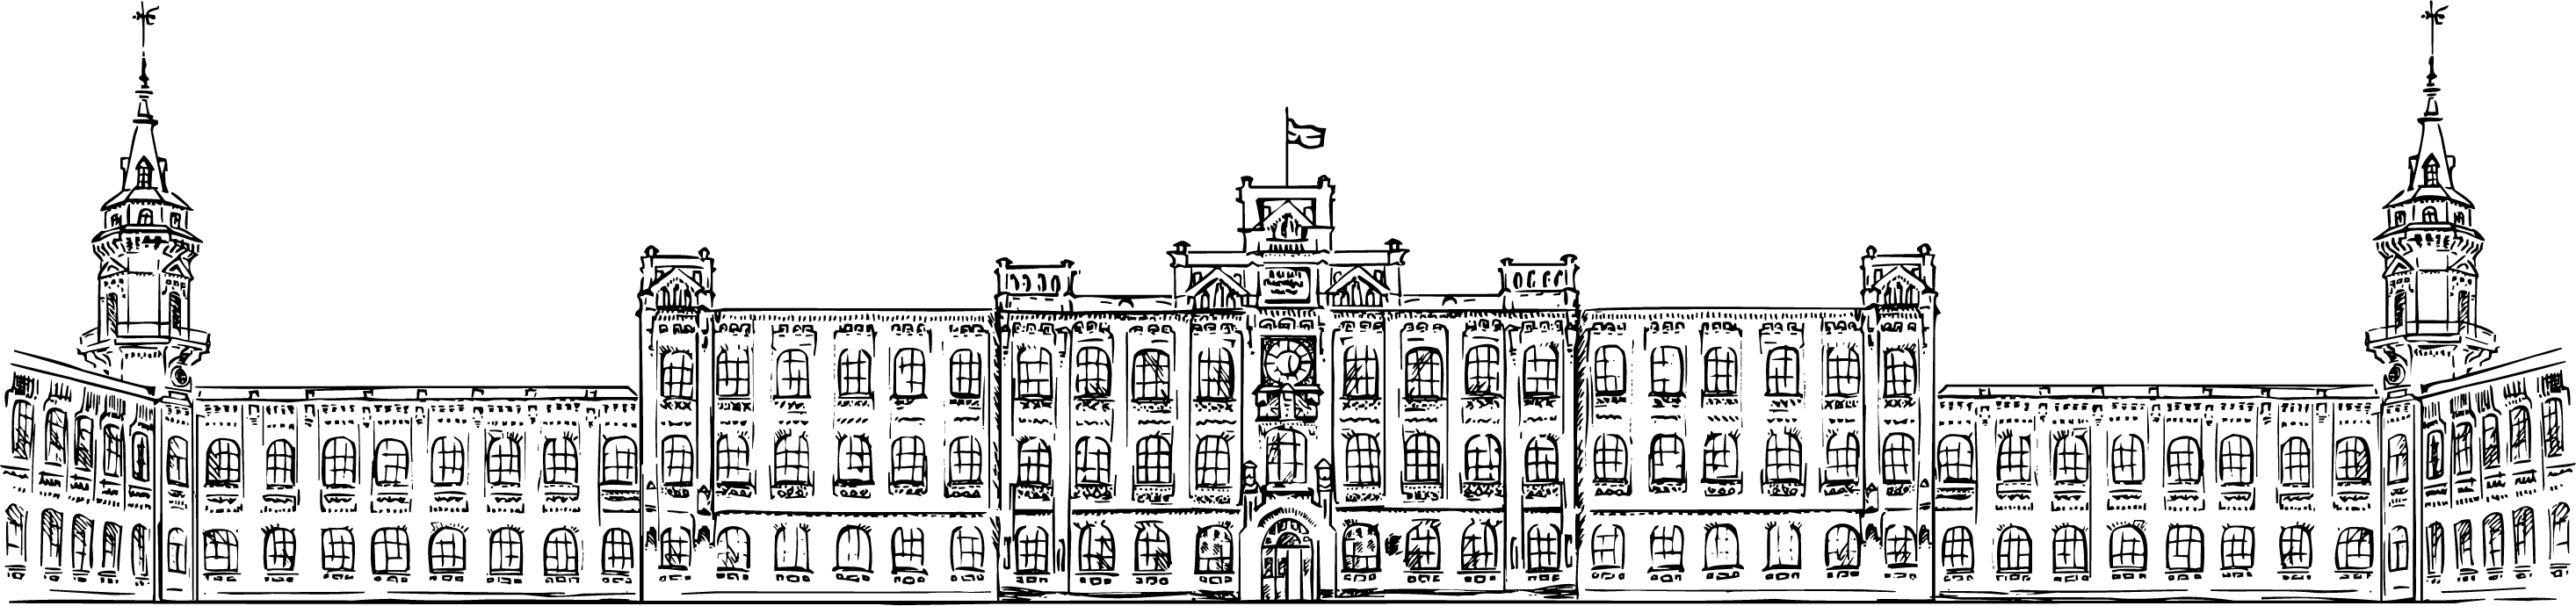
\includegraphics[width=0.7\textwidth]{../../TITLES/letterhead.png}
    \end{center}

    \begin{center}
        \large Національний технічний університет України\\
        «Київський політехнічний інститут імені Ігоря Сікорського»\\[1em]
        Факультет інформатики та обчислювальної техніки\\
        Кафедра обчислювальної техніки
    \end{center}

    \vfill

    \begin{center}
        \textbf{\LARGE Цифрова схемотехніка}\\[2em]
        \textbf{\Large Домашня контрольна робота}\\[0.5em]
        «Розроблення модулів арифметико-логічних блоків»
    \end{center}

    \vfill

    \begin{flushright}
        Виконали: студенти 2 курсу ФІОТ, гр. ІО-41\\
        \textit{Давидчук А. М.}\\
        \textit{Дубров Д. О.}\\
        Залікова книжка № 4106\\[1em]
        Перевірив: \textit{Нікольський С.\,С.}
    \end{flushright}

    \vfill

    \begin{center}Київ --- 2026\end{center}
\end{titlepage}

\noindent
\textbf{\underline{Тема:}} «Розроблення модулів арифметико-логічних блоків».

\vspace{1em}

\noindent
\textbf{\underline{Мета роботи:}} розробити та дослідити роботу арифметико-логічного блока із загальними мікроопераціями, реалізувати формування ознак результату, виконати функціональне моделювання за допомогою тестового рівня коду та додатково реалізувати нормалізацію результату шляхом зсуву праворуч на один розряд.

\begin{center}
    \textbf{\Large Хід роботи}
\end{center}

\section*{Визначення варіанта}

Номер залікової книжки: 4106. У двійковому вигляді:
\[
4106_{10}=0001\,0000\,0000\,1010_2.
\]
Звідси:
\[
h_7=0,\ h_6=0,\ h_5=0,\ h_4=1,\ h_3=0,\ h_2=1,\ h_1=0.
\]

За таблицею вибору варіанта для розроблення АЛБ для набору
\[
h_4=1,\ h_2=1,\ h_3=0,\ h_1=0
\]
отримано такий набір мікрооперацій:

\begin{table}[H]
    \centering
    \renewcommand{\arraystretch}{1.3}
    \begin{tabular}{|c|c|}
        \hline
        \textbf{ALB\_MI $I_4I_3$} & \textbf{Мікрооперація} \\
        \hline
        00 & $R \vee S$ \\
        \hline
        01 & $R + S + CI$ \\
        \hline
        10 & $S - R - 1 + CI$ \\
        \hline
        11 & $R \vee S$ \\
        \hline
    \end{tabular}
    \caption{Мікрооперації АЛБ за варіантом}
\end{table}

\section*{Структура проєкту}

Проєкт реалізовано у каталозі \texttt{Davydchuk\_Dubrov\_Mega\_Lab\_ALB}. Для моделювання використано підхід з окремим тестовим рівнем, який складається з генератора вхідних параметрів, базової моделі та модуля перевірки.

\begin{table}[H]
    \centering
    \renewcommand{\arraystretch}{1.25}
    \begin{tabular}{|p{0.32\textwidth}|p{0.56\textwidth}|}
        \hline
        \textbf{Файл} & \textbf{Призначення} \\
        \hline
        \texttt{src/alb.v} & основний модуль АЛБ із вхідними регістрами, формуванням результату, ознак та нормалізованого виходу \\
        \hline
        \texttt{sim/alb\_ref.v} & еталонна математична модель для порівняння \\
        \hline
        \texttt{sim/stimulus.v} & генератор тестових векторів \\
        \hline
        \texttt{sim/checker.v} & модуль автоматичної перевірки результатів \\
        \hline
        \texttt{sim/top.v} & верхній модуль тестового рівня \\
        \hline
        \texttt{sim/run.do} & скрипт запуску компіляції та симуляції в ModelSim \\
        \hline
    \end{tabular}
    \caption{Склад проєкту}
\end{table}

Модуль параметризовано за розрядністю \texttt{WIDTH}. У тестовому рівні використано \texttt{WIDTH = 12}, щоб дослідити приклади з розрядністю, достатньою для знакового результату і нормалізації.

\begin{figure}[H]
    \centering
    \resizebox{\textwidth}{!}{
    \begin{tikzpicture}[
        font=\small,
        reg/.style={draw, rectangle, align=center, minimum width=1.35cm, minimum height=0.62cm},
        core/.style={draw, rectangle, align=center, minimum width=3.8cm, minimum height=4.35cm},
        block/.style={draw, rectangle, align=center, minimum width=2.25cm, minimum height=0.9cm},
        signal/.style={-Latex, thin},
        bus/.style={-Latex, very thick},
        tap/.style={thin}
    ]
        \draw[bus] (0,0) -- (0,-5.0) node[below] {$R$};
        \draw[bus] (0.85,0) -- (0.85,-5.0) node[below] {$S$};
        \draw[bus] (1.90,0) -- (1.90,-5.0) node[below] {$CI$};
        \draw[bus] (3.10,0) -- (3.10,-5.0) node[below] {$ALB\_MI$};
        \node[above] at (0,0) {\scriptsize 12};
        \node[above] at (0.85,0) {\scriptsize 12};
        \node[above] at (1.90,0) {\scriptsize 1};
        \node[above] at (3.10,0) {\scriptsize 2};

        \node[reg] (rga) at (4.80,-0.65) {$RgA$};
        \node[reg] (rgb) at (4.80,-1.65) {$RgB$};
        \node[reg] (rgci) at (4.80,-2.65) {$RgCI$};
        \node[reg] (rgmi) at (4.80,-3.65) {$RgMI$};

        \draw[signal] (0,-0.65) -- (rga.west);
        \draw[signal] (0.85,-1.65) -- (rgb.west);
        \draw[signal] (1.90,-2.65) -- (rgci.west);
        \draw[signal] (3.10,-3.65) -- (rgmi.west);

        \node[core] (core) at (8.05,-2.35) {};
        \node[align=center] at (8.05,-0.85) {\textbf{Комбінаційна}\\\textbf{частина АЛБ}};
        \node[align=left] at (8.05,-2.20) {
            $00:\ R \vee S$\\
            $01:\ R + S + CI$\\
            $10:\ S - R - 1 + CI$\\
            $11:\ R \vee S$
        };
        \node[align=center] at (8.05,-3.80) {MX вибору\\мікрооперації};

        \draw[bus] (rga.east) -- node[above]{\scriptsize 12} (core.west |- rga.east);
        \draw[bus] (rgb.east) -- node[above]{\scriptsize 12} (core.west |- rgb.east);
        \draw[signal] (rgci.east) -- node[above]{\scriptsize 1} (core.west |- rgci.east);
        \draw[signal] (rgmi.east) -- node[above]{\scriptsize sel} (core.west |- rgmi.east);

        \coordinate (res) at (11.85,-2.35);
        \draw[bus] (core.east) -- node[above,pos=0.55]{\scriptsize 12} node[below,pos=0.55,yshift=-1pt] {$F\_ALB$} (res);

        \node[block] (flags) at (13.85,-1.15) {Логіка\\ознак};
        \node[block] (norm) at (13.85,-3.65) {Постпроцесор\\нормалізації};

        \draw[signal] (res) |- (flags.west);
        \draw[signal] (res) |- (norm.west);
        \draw[signal] (flags.south) -- node[right]{\scriptsize $VO,NO$} (norm.north);

        \draw[signal] (flags.east) -- ++(0.85,0) node[right] {$CO$};
        \draw[signal] (flags.east) -- ++(0.40,0) |- ++(0.45,-0.32) node[right] {$VO$};
        \draw[signal] (flags.east) -- ++(0.40,0) |- ++(0.45,-0.64) node[right] {$NO$};
        \draw[signal] (flags.east) -- ++(0.40,0) |- ++(0.45,-0.96) node[right] {$ZO$};
        \draw[bus] (norm.east) -- node[above]{\scriptsize 12} ++(0.95,0) node[right] {$F\_NORM$};
        \draw[signal] (norm.east) -- ++(0.40,0) |- ++(0.55,-0.42) node[right] {$NORM\_RIGHT$};

        \draw[tap] (0,-0.65) -- ++(0.12,0.12);
        \draw[tap] (0.85,-1.65) -- ++(0.12,0.12);
        \draw[tap] (1.90,-2.65) -- ++(0.12,0.12);
        \draw[tap] (3.10,-3.65) -- ++(0.12,0.12);
    \end{tikzpicture}}
    \caption{Структурна схема розробленого АЛБ}
\end{figure}

\section*{Розподіл виконання роботи}

Роботу виконано спільно. Основну функціональну частину проєкту, тобто визначення варіанта, розроблення структури АЛБ, реалізацію мікрооперацій та формування ознак результату, виконав Давидчук А. М. Дубров Д. О. виконав тестову частину роботи: підготовку тестових векторів, еталонної моделі, автоматичної перевірки результатів, запуск функціонального моделювання в ModelSim та оформлення результатів у звіті.

\section*{Реалізація АЛБ}

Вхідні аргументи \texttt{A\_ALB}, \texttt{B\_ALB}, перенос \texttt{CI} та мікроінструкція \texttt{ALB\_MI} записуються у буферні регістри за фронтом \texttt{clock}. При активному нулі \texttt{resetb} регістри очищуються.

Для мікрооперації \texttt{10} вираз
\[
S - R - 1 + CI
\]
реалізовано через доповняльний код:
\[
S - R - 1 + CI = S + \overline{R} + CI.
\]

Ознаки формуються так:
\begin{itemize}
    \item \texttt{CO} --- перенос за межі розрядної сітки;
    \item \texttt{VO} --- переповнення для арифметичних операцій у доповняльному коді;
    \item \texttt{NO} --- знак результату, тобто старший біт;
    \item \texttt{ZO} --- рівність результату нулю;
    \item \texttt{NORM\_RIGHT} --- необхідність нормалізації праворуч.
\end{itemize}

Повну реалізацію вибору мікрооперацій наведено у лістингу файлу \texttt{src/alb.v}. У звіті цей код підтягується без дублювання вручну через команду \texttt{\textbackslash inputminted}.

Додаткове завдання реалізовано як постпроцесор. Якщо встановлено ознаку переповнення і порушено нормалізацію ліворуч, результат зсувається на один розряд праворуч зі збереженням знакового біта:

Повний код постпроцесора також наведено у лістингу \texttt{src/alb.v}.

\section*{Тестовий рівень}

Тестовий рівень побудовано за структурою:
\[
\text{Stimulus} \rightarrow \text{DUT} \parallel \text{Reference model} \rightarrow \text{Checker}.
\]

\texttt{stimulus.v} подає на вхід АЛБ різні комбінації \texttt{ALB\_MI}, аргументів та переносу \texttt{CI}. \texttt{alb\_ref.v} обчислює очікуваний результат математично. \texttt{checker.v} порівнює результат основного модуля з еталонною моделлю.

Команда запуску симуляції в ModelSim:

\begin{minted}{text}
cd Davydchuk_Dubrov_Mega_Lab_ALB/sim
vsim -do run.do
\end{minted}

Для консольного запуску:

\begin{minted}{text}
vsim -c -do run.do
\end{minted}

\section*{Результати моделювання}

Під час моделювання перевірено логічні операції, додавання, віднімання у доповняльному коді, формування ознак і роботу нормалізації. Нижче наведено фрагмент Transcript ModelSim, у якому видно компіляцію модулів, запуск верхнього рівня та проходження автоматичної перевірки:

\begin{minted}{text}
# do run.do
# vlog ../src/alb.v alb_ref.v stimulus.v checker.v top.v
# -- Compiling module alb
# -- Compiling module alb_ref
# -- Compiling module stimulus
# -- Compiling module checker
# -- Compiling module top
# Top level modules:
#   top
# vsim work.top
# Loading work.top
# Loading work.alb
# Loading work.alb_ref
# Loading work.stimulus
# Loading work.checker
# run -all
# 80000 correct F=010000100101 FN=010000100101 C=0 V=0 N=0 Z=0 NR=0
# 100000 correct F=000111011010 FN=000111011010 C=1 V=0 N=0 Z=0 NR=0
# 110000 correct F=100100000000 FN=110010000000 C=0 V=1 N=1 Z=0 NR=1
# 120000 correct F=001100000000 FN=001100000000 C=1 V=1 N=0 Z=0 NR=0
# 130000 correct F=000000000010 FN=000000000010 C=1 V=0 N=0 Z=0 NR=0
# 140000 correct F=111111111110 FN=111111111110 C=0 V=0 N=1 Z=0 NR=0
# 170000 correct F=000000000000 FN=000000000000 C=1 V=0 N=0 Z=1 NR=0
# TEST PASSED
# ** Note: $finish    : stimulus.v(58)
#    Time: 245 ns  Iteration: 1  Instance: /top/stim
\end{minted}

\begin{table}[H]
    \centering
    \renewcommand{\arraystretch}{1.25}
    \begin{tabular}{|c|c|c|c|c|c|c|}
        \hline
        \textbf{Операція} & \textbf{F} & \textbf{F\_NORM} & \textbf{CO} & \textbf{VO} & \textbf{NO} & \textbf{ZO} \\
        \hline
        $R+S+CI$ & 100100000000 & 110010000000 & 0 & 1 & 1 & 0 \\
        \hline
        $R+S+CI$ & 001100000000 & 001100000000 & 1 & 1 & 0 & 0 \\
        \hline
        $S-R-1+CI$ & 000000000010 & 000000000010 & 1 & 0 & 0 & 0 \\
        \hline
        $S-R-1+CI$ & 111111111110 & 111111111110 & 0 & 0 & 1 & 0 \\
        \hline
        $R+S+CI$ & 000000000000 & 000000000000 & 1 & 0 & 0 & 1 \\
        \hline
    \end{tabular}
    \caption{Приклади формування ознак}
\end{table}

У першому прикладі утворено переповнення і порушення нормалізації ліворуч, тому постпроцесор сформував \texttt{NORM\_RIGHT = 1} і виконав зсув результату праворуч. В інших наведених прикладах показано формування ознак переносу, знаку та нульового результату.

\begin{figure}[H]
    \centering
    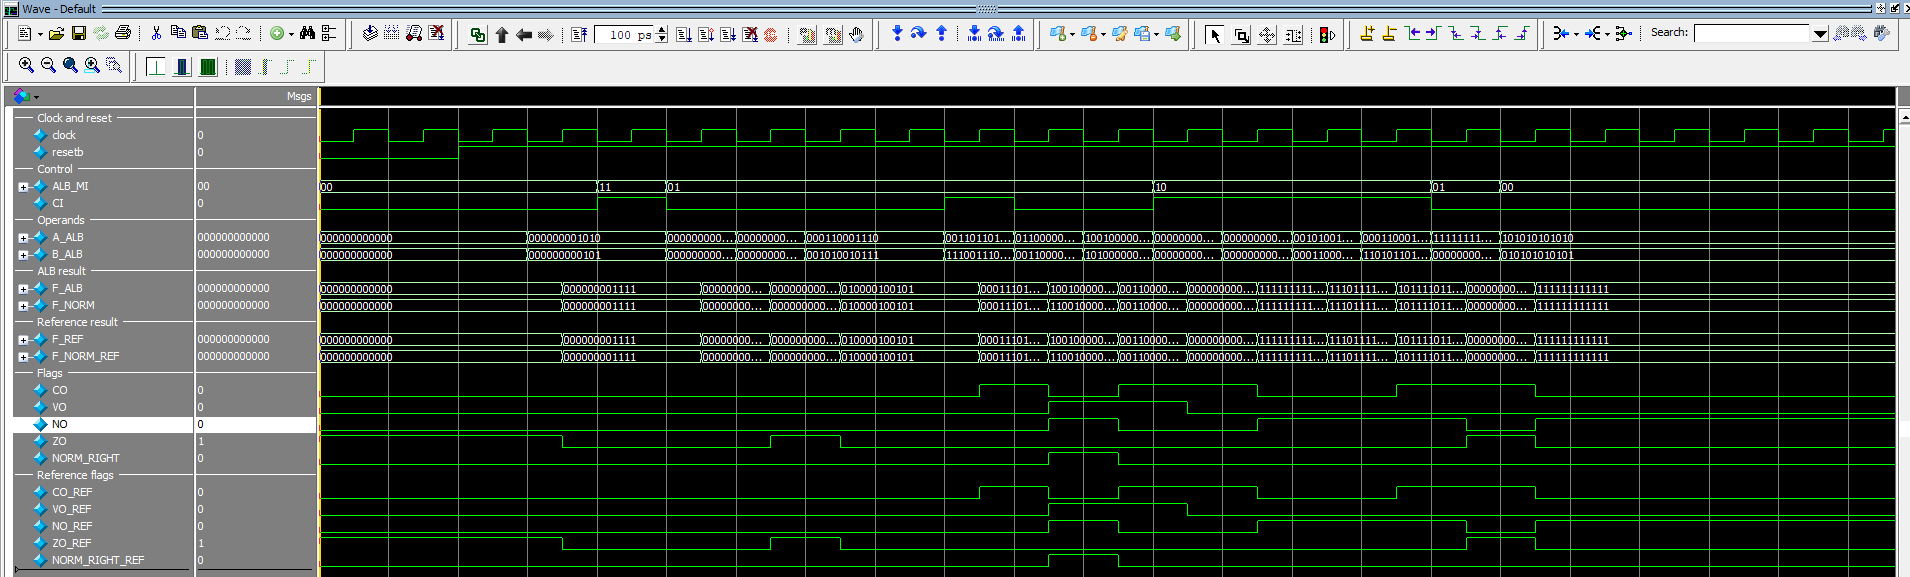
\includegraphics[width=\textwidth]{media/wave_window.png}
    \caption{Часова діаграма роботи АЛБ у ModelSim}
\end{figure}

\begin{figure}[H]
    \centering
    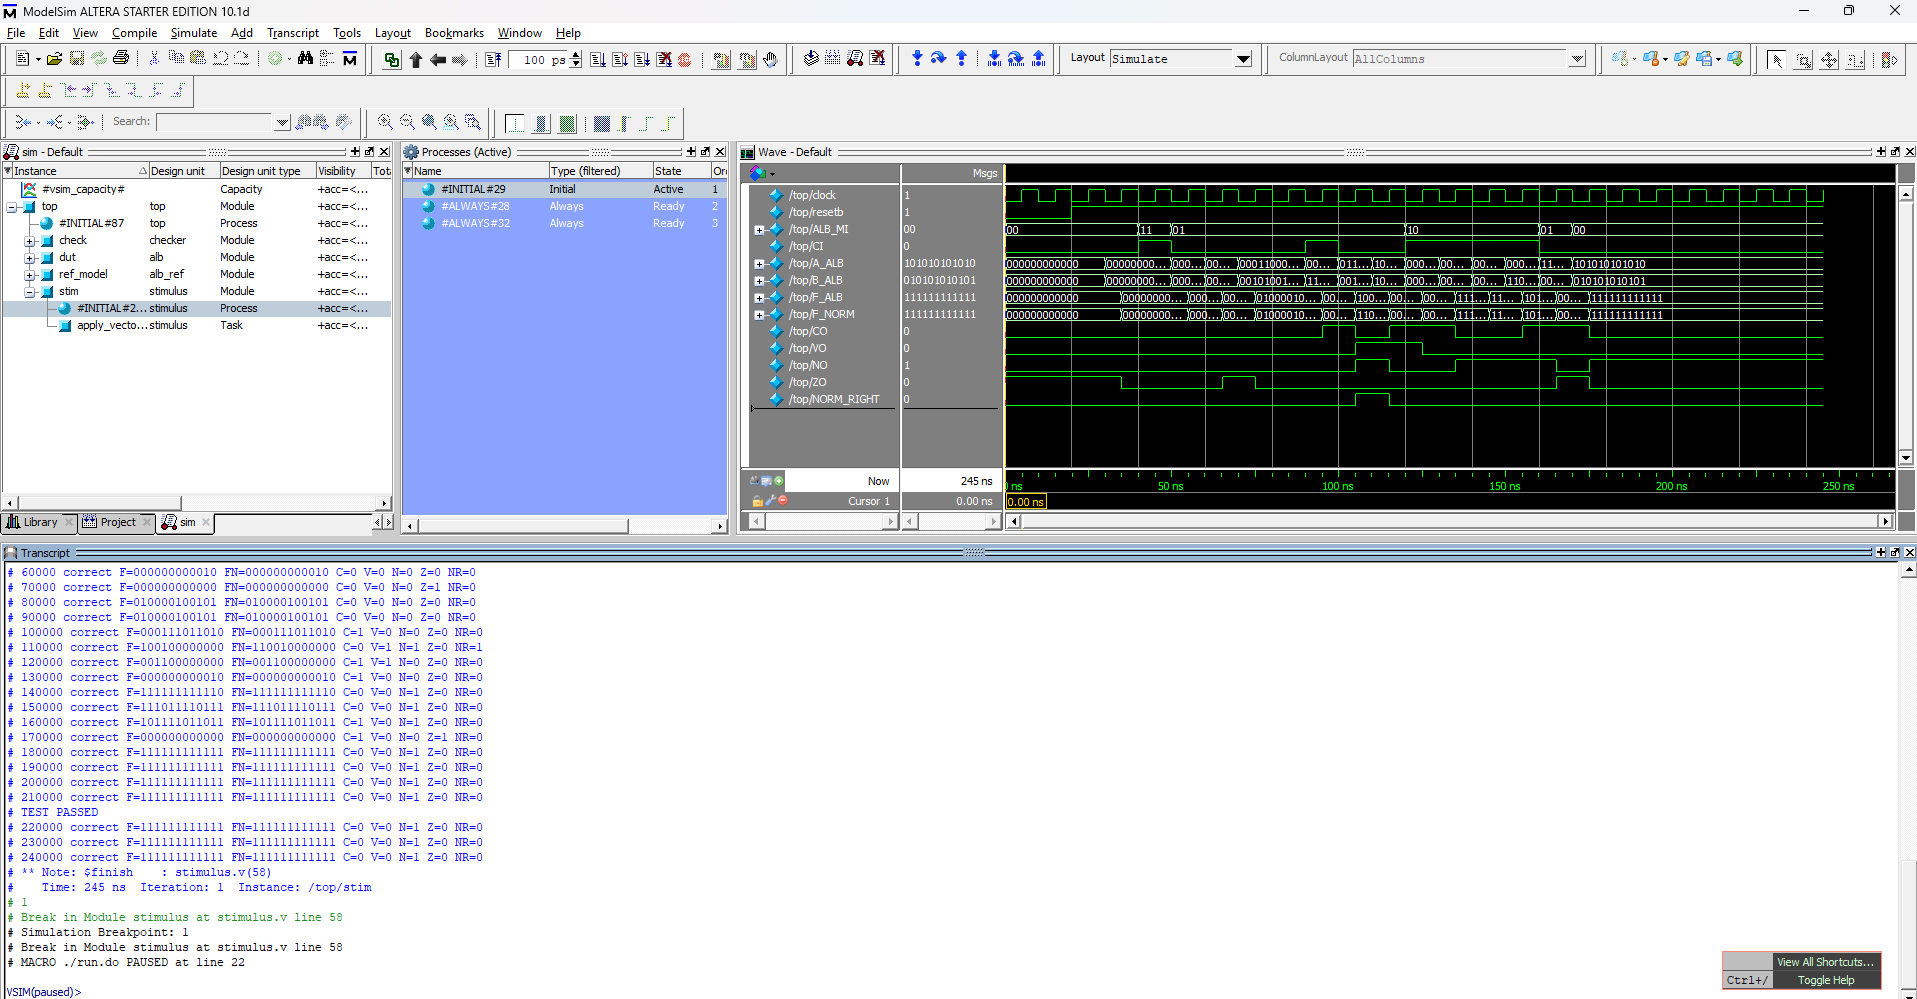
\includegraphics[width=\textwidth]{media/all_window.png}
    \caption{Загальний вигляд середовища ModelSim після завершення симуляції}
\end{figure}

\section*{Лістинг програмного коду}

Нижче наведено повний код модулів і скриптів, які використовуються для функціонального моделювання АЛБ.

\begin{itemize}
    \item \texttt{src/alb.v} --- основний модуль АЛБ. У ньому реалізовано вхідні буферні регістри, вибір мікрооперації за сигналом \texttt{ALB\_MI}, формування результату \texttt{F\_ALB}, ознак \texttt{CO}, \texttt{VO}, \texttt{NO}, \texttt{ZO}, а також бонусний постпроцесор нормалізації з виходами \texttt{F\_NORM} і \texttt{NORM\_RIGHT}.
    \item \texttt{sim/alb\_ref.v} --- еталонна математична модель. Вона описує ті самі мікрооперації без структурної деталізації АЛБ і використовується для порівняння з основним модулем.
    \item \texttt{sim/stimulus.v} --- генератор тестових векторів. Він послідовно задає \texttt{A\_ALB}, \texttt{B\_ALB}, \texttt{CI} та \texttt{ALB\_MI}, щоб перевірити логічні операції, додавання, віднімання, перенос, переповнення, знак, нульовий результат і нормалізацію.
    \item \texttt{sim/checker.v} --- модуль автоматичної перевірки. Він порівнює результат основного АЛБ з еталонною моделлю та виводить \texttt{error} у разі розбіжності або \texttt{TEST PASSED}, якщо всі перевірки пройдено.
    \item \texttt{sim/top.v} --- верхній модуль тестового рівня. Він з'єднує основний АЛБ, еталонну модель, генератор тестів і модуль перевірки, а також формує сигнали \texttt{clock} і \texttt{resetb}.
    \item \texttt{sim/run.do} --- основний скрипт ModelSim. Він компілює файли, запускає симуляцію, додає основні сигнали на часову діаграму та виконує моделювання до завершення тесту.
    \item \texttt{sim/wave\_pretty.do} --- допоміжний скрипт для оформлення часових діаграм. Він групує сигнали, додає сигнали еталонної моделі та налаштовує вигляд вікна Wave для створення зрозумілого скріншоту.
\end{itemize}

\subsection*{\texttt{src/alb.v}}

\inputminted{verilog}{Davydchuk_Dubrov_Mega_Lab_ALB/src/alb.v}

\subsection*{\texttt{sim/alb\_ref.v}}

\inputminted{verilog}{Davydchuk_Dubrov_Mega_Lab_ALB/sim/alb_ref.v}

\subsection*{\texttt{sim/stimulus.v}}

\inputminted{verilog}{Davydchuk_Dubrov_Mega_Lab_ALB/sim/stimulus.v}

\subsection*{\texttt{sim/checker.v}}

\inputminted{verilog}{Davydchuk_Dubrov_Mega_Lab_ALB/sim/checker.v}

\subsection*{\texttt{sim/top.v}}

\inputminted{verilog}{Davydchuk_Dubrov_Mega_Lab_ALB/sim/top.v}

\subsection*{\texttt{sim/run.do}}

\inputminted{text}{Davydchuk_Dubrov_Mega_Lab_ALB/sim/run.do}

\subsection*{\texttt{sim/wave\_pretty.do}}

\inputminted{text}{Davydchuk_Dubrov_Mega_Lab_ALB/sim/wave_pretty.do}

\section*{Висновок}

У ході виконання домашньої контрольної роботи було розроблено параметризований АЛБ відповідно до варіанта, визначеного за номером залікової книжки 4106. Реалізовано мікрооперації $R \vee S$, $R + S + CI$ та $S - R - 1 + CI$, передбачено вхідні буферні регістри, сформовано ознаки \texttt{CO}, \texttt{VO}, \texttt{NO}, \texttt{ZO}.

Для перевірки створено тестовий рівень, що складається з генератора вхідних даних, еталонної математичної моделі та модуля автоматичної перевірки. Функціональне моделювання в ModelSim підтвердило відповідність результатів АЛБ еталонній моделі. Додатково реалізовано постпроцесор нормалізації, який за потреби виконує зсув результату на один розряд праворуч.

\end{document}
